\documentclass{amsart}
\usepackage{graphicx}
\graphicspath{{./}}
\usepackage{hyperref}
\usepackage{csvsimple}
\usepackage{longtable}
\usepackage{lscape}
\usepackage{epigraph}
\title{Analysis Of Ethnicity Effects on Confidence In Government}
\author{Zulfikar Moinuddin Ahmed}
\date{\today}
\begin{document}
\maketitle

\section{Novel Analysis}

We are interested in ethnicity effects on confidence in government.  We want to do this in several ways.  Unlike in the moral questions here we have some variation and we want thus to consider the variation multiple ways.

Of course straightforward statistical analysis of the groupings -- in this case 1,2,3,4-- is nice.  But we are also interested in embedding each ethnicity curve into the GHD space and attempting to examine variation in the parameter space of GHD.  We do this because we believe there is value in understanding continuous deformations and other analytical considerations.

\section{Line Plots}

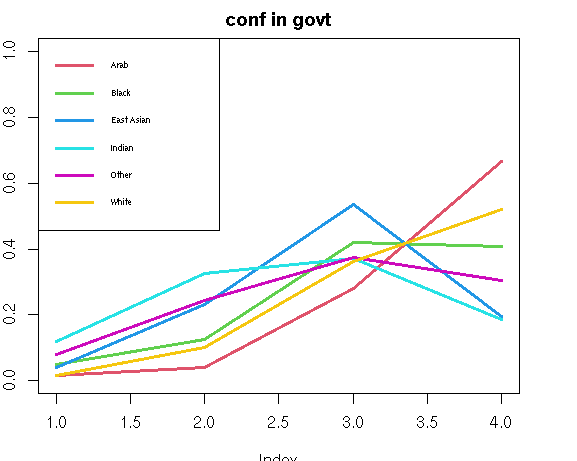
\includegraphics[scale=0.8]{confgovt.png}

Here 1=Great Deal and 4=None at all for confidence in government.  We can easily detect tighter bounds on the higher confidence.

[Put Basic Analysis]

Now the shape of the curves are different, however, and I want to capture the differences in a meaningful manner.  This we will attempt to do using GHD fits in the next section.

\section{Estimated GHD Parameters}

% latex table generated in R 4.0.3 by xtable 1.8-4 package
% Sun May 16 01:47:53 2021
\begin{table}[ht]
\centering
\begin{tabular}{rlrrrrr}
  \hline
 & eth & lambda & mu & sigma & gamma & alpha.bar \\ 
  \hline
1 & Arab & 1.735 & 4.611 & 0.001 & -1.010 & 0.000 \\ 
  2 & Black & -76.436 & 11.488 & 0.001 & -8.160 & 46.228 \\ 
  3 & East Asian & -47.434 & 8.530 & 0.001 & -5.666 & 31.043 \\ 
  4 & Indian & -276.043 & 21.004 & 0.001 & -18.413 & 167.434 \\ 
  5 & Other & -51.420 & 11.346 & 0.001 & -8.414 & 34.632 \\ 
  6 & White & 2.521 & 4.787 & 0.001 & -1.443 & 0.000 \\ 
   \hline
\end{tabular}
\end{table}


\section{Wiener Process Is Not Important to Nature}

When I was a graduate student at Columbia, I did study Ioannis Karatzas' book and then I went to work with Daniel Stroock.  But that was 1996-1999 a long long time ago.  In the intervening years, I was just thinking about Daniel Stroock's comments about the lecture on Levy Processes that illuminated him during his early career at Courant.  Well, the Levy Processes that matter for Nature are those associated with Generalised Hyperbolic Distributions and not Wiener Processes.  I am certain of this, and these fits you see get me closer to proving this.  I believe GHD are universal noise and are infinitely more important than Wiener Processes and Brownian Motion and Fractional Brownian Motion and all that.  These are Nature-sensitive, GHD-Levy Processes, and their theory does not really exist yet.  

\section{Caution Regarding Interpretation}

I do not know how to interpret these numbers yet, so I will leave their interpretation for the future.  Their interpretation will, I believe, open a new door of Man's Understanding of Nature because the not-yet-existent theory of GHD Levy processes will tell us a dynamical tale behind these distributions, and that is the rich mine into deeper understanding of Human Race Behaviour.

At a distance, this looks rather sketchy.  But it's not.  It's deep.  And this is why there are any geometric fits here at all.  This is where we want to go.  We want a deeper merging of Levy Process Theory for GHD and Social Sciences.

\section{Levy Process Model}

We hypothesize that there exists for each ethnicity a Levy Process where the equilibrium distribution is $\delta_e(x)$ where $e$ represents ethnicity.  Associated with this is a pure jump Levy process $X_e(t)$.  The distributions are Barndorff-Nielsen with fixed parameters we have estimated.  

This $X_e(t)$ is the ethnicity $e$ aggregate of a continuous variable taking values in $\mathbf{R}$. 

This is the idea behind a scientific model. We want to consider the ideas lightly until it produces a firm scientific theory.

Let us pretend that  time begins in the Dawn of Civilisation, say Mesopotamia, 3100 BC when written history began.  Then for whatever reason, the distribution of confidence in government reaches an equilibrium and so there is this $\delta_e(x)$ distribution on any nontrivial sample population.

The Levy process operates on the whole ethnicity $e$ in the world. 

This is not a scientific model yet, but it gives a bit more context, by introducing a continuous time Levy process model.

\section{Levy Process Models at Global Population Level}

My Markov Moral Model succeeded and is a Markov Chain model.  But there the chain was across morals.  Here we have at our disposal actual time. 

This is a good idea.  
 
\end{document}

